
% Template for Elsevier CRC journal article
% version 1.1 dated 16 March 2010

% This file (c) 2009-10 Elsevier Ltd.  Modifications may be freely made,
% provided the edited file is saved under a different name

% This file contains modifications for Nuclear Physics B Proceedings Supplement

% Changes since version 1.0
% - elsarticle class option changed from 1p to 3p (to better reflect CRC layout)
%

%-----------------------------------------------------------------------------------

%% This template uses the elsarticle.cls document class and the extension package ecrc.sty
%% For full documentation on usage of elsarticle.cls, consult the documentation "elsdoc.pdf"
%% Further resources available at http://www.elsevier.com/latex

%-----------------------------------------------------------------------------------

%%%%%%%%%%%%%%%%%%%%%%%%%%%%%%%%%%%%%%%%%%%%%%
%%%%%%%%%%%%%%%%%%%%%%%%%%%%%%%%%%%%%%%%%%%%%%
%%                                          %%
%% Important note on usage                  %%
%% -----------------------                  %%
%% This file must be compiled with PDFLaTeX %%
%% Using standard LaTeX will not work!      %%
%%                                          %%
%%%%%%%%%%%%%%%%%%%%%%%%%%%%%%%%%%%%%%%%%%%%%%
%%%%%%%%%%%%%%%%%%%%%%%%%%%%%%%%%%%%%%%%%%%%%%

%% The '3p' and 'times' class options of elsarticle are used for Elsevier CRC
\documentclass[3p,times,twocolumn]{elsarticle}

%% The `ecrc' package must be called to make the CRC functionality available
\usepackage{ecrc}

%% The ecrc package defines commands needed for running heads and logos.
%% For running heads, you can set the journal name, the volume, the starting page and the authors

%% set the volume if you know. Otherwise `00'
\volume{00}

%% set the starting page if not 1
\firstpage{1}

%% Give the name of the journal
\journalname{Nuclear Physics B Proceedings Supplement}

%% Give the author list to appear in the running head
%% Example \runauth{C.V. Radhakrishnan et al.}
\runauth{}

%% The choice of journal logo is determined by the \jid and \jnltitlelogo commands.
%% A user-supplied logo with the name <\jid>logo.pdf will be inserted if present.
%% e.g. if \jid{yspmi} the system will look for a file yspmilogo.pdf
%% Otherwise the content of \jnltitlelogo will be set between horizontal lines as a default logo

%% Give the abbreviation of the Journal.
\jid{nuphbp}

%% Give a short journal name for the dummy logo (if needed)
\jnltitlelogo{Nuclear Physics B Proceedings Supplement}

%% Hereafter the template follows `elsarticle'.
%% For more details see the existing template files elsarticle-template-harv.tex and elsarticle-template-num.tex.

%% Elsevier CRC generally uses a numbered reference style
%% For this, the conventions of elsarticle-template-num.tex should be followed (included below)
%% If using BibTeX, use the style file elsarticle-num.bst

%% End of ecrc-specific commands
%%%%%%%%%%%%%%%%%%%%%%%%%%%%%%%%%%%%%%%%%%%%%%%%%%%%%%%%%%%%%%%%%%%%%%%%%%

%% The amssymb package provides various useful mathematical symbols
\usepackage{amssymb}
%% The amsthm package provides extended theorem environments
%% \usepackage{amsthm}

%% The lineno packages adds line numbers. Start line numbering with
%% \begin{linenumbers}, end it with \end{linenumbers}. Or switch it on
%% for the whole article with \linenumbers after \end{frontmatter}.
%% \usepackage{lineno}

%% natbib.sty is loaded by default. However, natbib options can be
%% provided with \biboptions{...} command. Following options are
%% valid:

%%   round  -  round parentheses are used (default)
%%   square -  square brackets are used   [option]
%%   curly  -  curly braces are used      {option}
%%   angle  -  angle brackets are used    <option>
%%   semicolon  -  multiple citations separated by semi-colon
%%   colon  - same as semicolon, an earlier confusion
%%   comma  -  separated by comma
%%   numbers-  selects numerical citations
%%   super  -  numerical citations as superscripts
%%   sort   -  sorts multiple citations according to order in ref. list
%%   sort&compress   -  like sort, but also compresses numerical citations
%%   compress - compresses without sorting
%%
%% \biboptions{comma,round}

% \biboptions{}

% if you have landscape tables
\usepackage[figuresright]{rotating}

% put your own definitions here:
%   \newcommand{\cZ}{\cal{Z}}
%   \newtheorem{def}{Definition}[section]
%   ...

% add words to TeX's hyphenation exception list
%\hyphenation{author another created financial paper re-commend-ed Post-Script}

% declarations for front matter

\usepackage[table]{xcolor}

\begin{document}

\begin{frontmatter}

%% Title, authors and addresses

%% use the tnoteref command within \title for footnotes;
%% use the tnotetext command for the associated footnote;
%% use the fnref command within \author or \address for footnotes;
%% use the fntext command for the associated footnote;
%% use the corref command within \author for corresponding author footnotes;
%% use the cortext command for the associated footnote;
%% use the ead command for the email address,
%% and the form \ead[url] for the home page:
%%
%% \title{Title\tnoteref{label1}}
%% \tnotetext[label1]{}
%% \author{Name\corref{cor1}\fnref{label2}}
%% \ead{email address}
%% \ead[url]{home page}
%% \fntext[label2]{}
%% \cortext[cor1]{}
%% \address{Address\fnref{label3}}
%% \fntext[label3]{}

\dochead{}
%% Use \dochead if there is an article header, e.g. \dochead{Short communication}

\title{Search for heavy resonances decaying to bosons\\ with the ATLAS and CMS detectors}

%% use optional labels to link authors explicitly to addresses:
%% \author[label1,label2]{<author name>}
%% \address[label1]{<address>}
%% \address[label2]{<address>}

\author{}

\address{}

\begin{abstract}
This document summarizes the searches for heavy resonances decaying to
massive bosons at the TeV mass scale. Results are based on data corresponding to an integrated luminosity
up to about 20 inverse femtobarns recorded in proton-proton collisions at
$\sqrt{s} = 8$ TeV with the ATLAS and CMS detector at the CERN LHC. 
The bosons coming from the resonance decay can be W, Z, 
or the standard model Higgs. Several final states are
considered: fully leptonic, leptons plus jets, 
and fully hadronic final sates. Techniques aiming at identifying jet
substructures are used to analyze signal events in which the
hadronization products from the decay of highly boosted W or Z 
bosons are contained within a single reconstructed jet. 
No significant excess above the standard model prediction is observed
in data. Upper limits on the production of diboson resonances are 
set as a function of the resonance mass and width. 
These searches provide the most stringent direct limits to date on the production of these
hypothesized TeV-scale resonances. 
\end{abstract}

\begin{keyword}
%% keywords here, in the form: keyword \sep keyword
%% MSC codes here, in the form: \MSC code \sep code
%% or \MSC[2008] code \sep code (2000 is the default)
Physics Beyond the Standard Model, New Resonances, LHC, CMS, Diboson, Higgs, Jet substructure
\end{keyword}

\end{frontmatter}

%%
%% Start line numbering here if you want
%%
% \linenumbers

%% main text
\section{Introduction}
\label{sec:introduction}
One century of experimental measurements and progress in theoretical
physics led to an extremely compact and elegant theory of fundamental
interactions between elementary particles, the standard model (SM). 
Its success in reproducing measurements from different experiments in
energy regimes spanning over several orders of magnitude is
astonishing. The relatively recent discovery of the Higgs boson (H)
at the CERN Large Hadronc Collider (LHC) is another confirmation of
the success of the SM. Still there are several open questions which
cannot be answered in the contest of the SM, of which some of the most
important ones are: {\it what is the dark matter?}, {\it what is the cause of the
matter-antimatter asymmetry in the universe?}, {\it what is the reason for
the large difference between the electroweak and the gravity scale?}

Looking for signs of new physics beyond the SM at the TeV scale might
help to answer some of these fundamental questions. One of the most
direct ways to find new physics at the TeV scale is to search for new resonances.
Colliding hadrons at the highest reachable energy to possibly create 
and study these new massive states has been a successful experimental
approach in particle physics during the last 50 years. 
%An historical, but relevant example: in early
%60s the collisions of hadrons reached
%a new energy frontier of $\sqrt{s}\sim$ GeV and new resonances were promptly discovered (see 
%as example the discoveries of $\rho(770)\rightarrow \pi\pi$~\cite{}, $K^{*}(892)\rightarrow
%$K$\pi$~\cite{}, $\phi(1020)\rightarrow KK$~\cite{}, and others in the few years
%after 1960). The known properties of pions and kaons (mass, decays,
%quantum numbers) were exploited to study these new particles.
%The same general experimental strategy can be
%applied at the LHC with the difference that the collider energy is
%much larger, thus allowing to study the production of heavy resonances
%in the TeV mass range. 
%These heavy resonances are typically
%unstable and we can detect them by looking at their decay products.
This document presents searches for heavy resonances decaying to SM
bosons. Results are based on data corresponding to an integrated luminosity
up to about 20 inverse femtobarns recorded in proton-proton collisions at
$\sqrt{s} = 8$ TeV with the ATLAS~\cite{1748-0221-3-08-S08003} 
and CMS~\cite{Chatrchyan:2008aa} detectors at the CERN LHC. 
The bosons coming from the resonance decay can be photon, W, Z, or H. 
One of the main advantages of these searches is the clean 
experimental signature, thanks to the known properties
and decay kinematics of the SM bosons. Diboson resonances
are also predicted in many model of new physics beyond the SM, such as
the sequential standard model extension~\cite{Altarelli:1989ff},
composite Higgs
models~\cite{Kaplan:1983fs,Contino:2006nn,Giudice:2007fh}, 
scenarios with extra 
dimensions~\cite{Randall:1999ee,Agashe:2007zd,Fitzpatrick:2007qr,Antipin:2007pi}, 
Technicolor~\cite{Susskind:1978ms,Lane:1999uh,Eichten:2007sx} and others.

In Section~\ref{sec:HH} we present searches for resonances that decay to
pairs of SM Higgs bosons. Section~\ref{sec:VV} summarises the results of
searches for resonances decaying to pairs of V bosons (where V
indicates either W or Z). 
Results of searches for heavy resonances decaying to 
$\gamma\gamma$~\cite{CMS:2014onr}, W$\gamma$/Z$\gamma$~\cite{Aad:2014fha}, and 
 HH/ZH in the multileptons and photons~\cite{Khachatryan:2014jya} final states 
are discussed in more details in other proceedings of this conference
(see M. Kenzie's, K. Terashi's, and O. Bondu’s proceedings).
%In Section~\ref{sec:Comparison} we compare the results of some of these
%searches using a benchmark theoretical model. 
In Section~\ref{sec:Conclusion} we conclude by summarizing the current status of the
diboson searches at LHC and we give some prospects for future studies
during the second run-phase of the LHC.

\section{HH Resonances}
\label{sec:HH}

Both ATLAS and CMS have searched for heavy resonances (X) decaying to
pairs of Higgs bosons in the $\rm{X}\rightarrow\rm{HH}\rightarrow \gamma\gamma\rm{bb}$ and $\rm{X}\rightarrow\rm{HH}\rightarrow 4\rm{b}$ final states. 
The $\gamma\gamma\rm{bb}$ channel is a powerful final state in which
to search for Higgs boson pair production, thanks to the large
$\rm{H}\rightarrow\rm{bb}$ branching ratio ($\sim$57\%), clean diphoton trigger,
excellent diphoton invariant mass resolution (about 1\% for the SM Higgs), and low
backgrounds. This channel is particularly important in search for
resonances with mass below 500 GeV. At higher resonance masses, the 4b channel
dominates the sensitivity to new physics thanks to the larger branching ratio.


\subsection{$\gamma\gamma\rm{bb}$ Channel}

The ATLAS $\gamma\gamma\rm{bb}$ analysis~\cite{Aad:2014yja} starts by requiring an
$\rm{H}\rightarrow \gamma\gamma$ candidate in the event, accordingly
with the standard model analysis. In addition two jets, identified as
coming from hadronization of b quarks (b-jets), are required with dijet
mass $95<m_{jj}<135$~GeV compatible with the Higgs boson
signature. Finally the mass of the $\gamma\gamma\rm{bb}$ system
($m_{\gamma\gamma\rm{bb}}$) is required to be consistent with the
hypothesised resonance mass ($m_X$). The search is performed as a counting 
experiment where the  $\gamma\gamma\rm{bb}$ requirement varies as a
function of $m_X$. The SM backgrounds are estimated from
$m_{\gamma\gamma}$ sidebands and events with less than 2 b-jets. 

The CMS $\gamma\gamma\rm{bb}$ selection~\cite{CMS:2014ipa} is conceptually similar to the
ATLAS one. A few differences in the analysis strategy are represented by the presence of
two separate event categories (1 or 2 b-jets), lower requirement on jet $p_{\rm{T}}$
(25 GeV instead of 35-55 GeV of the ATLAS search), and the use of a shape analysis (instead of a
counting experiment) in either the $m_{\gamma\gamma}$ or the
$m_{\gamma\gamma\rm{bb}}$ distribution, depending on the resonance
mass tested.

The ATLAS search observes a broad excess of events compared to SM
predictions at a resonance mass around 300 GeV. The event distribution
does not seem consistent with the $m_{\gamma\gamma\rm{bb}}$ resolution
of a narrow resonance. Figure~\ref{fig:ATLAS_HH_ggbb} shows the upper limits on
production cross section times branching ratio as a function of the
resonance mass. The broad excess is visible within the 2$\sigma$ bands
of the expected limit. By visual comparison with the CMS results in
Figure~\ref{fig:CMS_HH_summary} (see the dark blue lines), after dividing the CMS limit by the factor
$\rm{BR(}\rm{HH}\rightarrow \gamma\gamma\rm{bb}\rm{)}\sim0.2\%$ to
match the y-axis scale in the two plots, we notice that the ATLAS excess seems to be excluded by
the CMS constraints on the same production cross section. The CMS
analysis also appear more sensitive than the ATLAS one, providing
expected upper limits about 50\% smaller.

\begin{figure}[htbp]
\centering
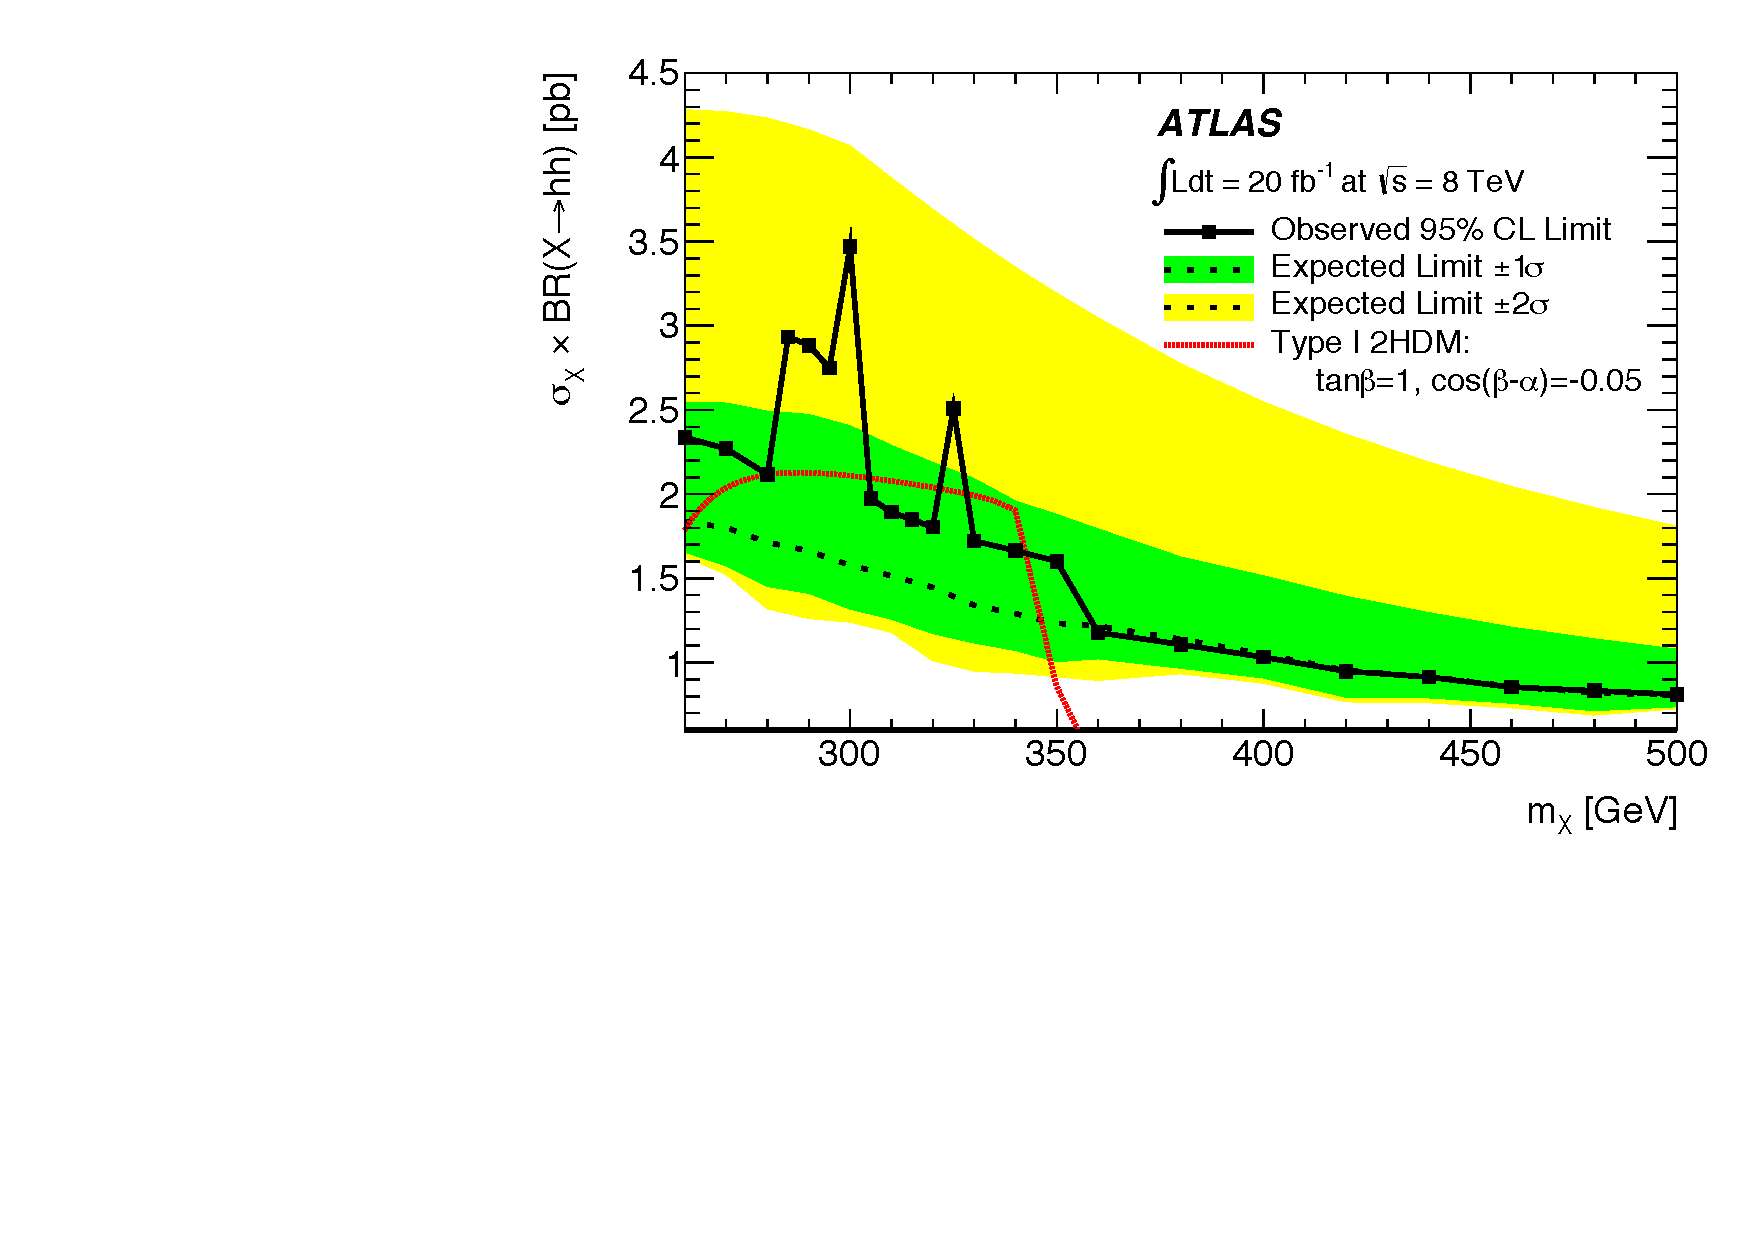
\includegraphics[width=8cm]{ATLAS_HH_ggbb_limit.pdf}
\caption{The ATLAS 95\% CL upper limits on the cross section times branching
  ratio of a narrow spin-0 resonance decaying to pairs of Higgs bosons
  in the $\gamma\gamma\rm{bb}$ final state as a function of $m_X$~\cite{Aad:2014yja}.}\label{fig:ATLAS_HH_ggbb}
\end{figure}

\begin{figure}[htbp]
\centering
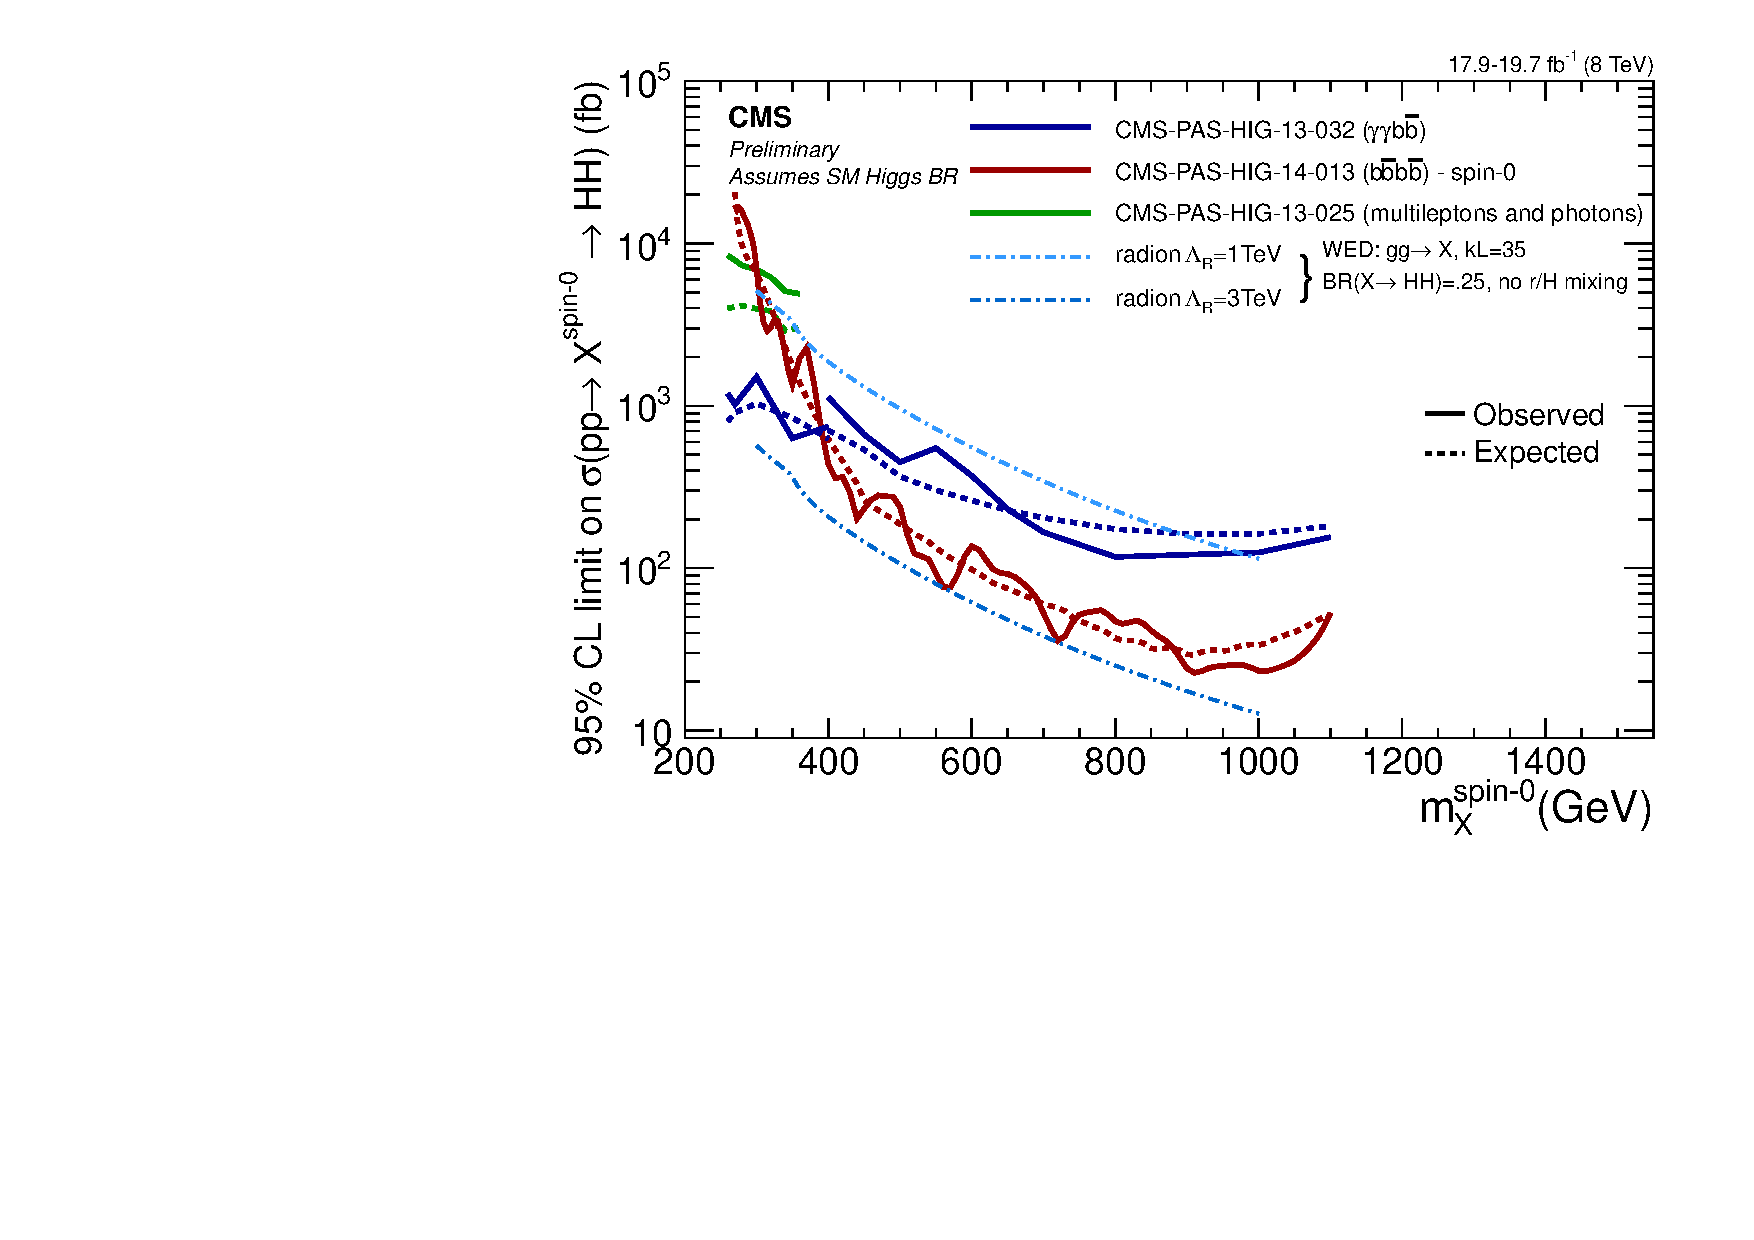
\includegraphics[width=8cm]{CMS_HH_summary.pdf}
\caption{The expected and observed upper limit of spin-0 X to HH
  production at 95\% CLs provided by combining the searches performed
  by the CMS experiment looking at the 4b (HIG-14-013)~\cite{CMS:2014eda}, $\gamma\gamma\rm{bb}$
  (HIG-13-032~\cite{CMS:2014ipa}), and multileptons and photons
  (HIG-13-025~\cite{Khachatryan:2014jya}) final
  states. Theoretical cross sections for the RS1-radion, with
  $\Lambda_R = 1$ and 3 TeV, kL = 35, and no radion-Higgs mixing are overlaid.}\label{fig:CMS_HH_summary}
\end{figure}

\subsection{4b Channel}
The ATLAS HH$\rightarrow$4b selection~\cite{Aad:2014yja} requires at least 4 b-jets with
$p_{\rm{T}}>40$~GeV. Two unique dijets (system of two jets) are formed
from the four highest-$p_{\rm{T}}$ b-tagged jets requiring for each
dijet system a maximum angular separation between the jets
($\Delta R=\sqrt{\Delta\phi^2+\Delta\eta^2}<1.5$)
and the $p_{\rm{T}}^{\rm{dijet}}>200$~GeV. A set of kinematic
requirements are applied in order to reduce the $\rm{t}\bar{\rm{t}}$
background, including a veto on extra jets in the event, as well as 
selections to isolate the $\rm{t}\bar{\rm{t}}$ decay kinematics.
After this selection, the dominant background is coming from QCD
multijet events. The QCD background is estimated from data using an
extrapolation from events with 2-bjets in the 4 b-jet signal
region. The 4b invariant mass resolution is of the order of 15\% for a
resonance mass of 1 TeV. No excess in data above the SM background
expectation is observed. Figure~\ref{fig:ATLAS_HH_4b_limit} shows the upper limits 
on production cross section for a bulk graviton~\cite{Agashe:2007zd} that decays to
HH in the 4b channel. The upper limits increase for resonance masses
above 1 TeV; in this mass range, the Higgs bosons from resonance decay
are highly boosted and their decay products are contained within a
single reconstructed jet. This causes an inefficiency in the 4b
selection, because it's not possible to reconstruct 4 resolved jets. 
Techniques aiming to solve this experimental issue will be discussed
later in Section~\ref{sec:JetSubstructure} in the contest of the VV searches. 

After the ICHEP2014 conference, the CMS collaboration released the
results of a similar HH search in 4b final state~\cite{CMS:2014eda}. The CMS
limit is shown in Fig.~\ref{fig:CMS_HH_summary} (red line). 
The sensitivities of the ATLAS and CMS analysis are comparable in the 
overlapping mass range between 0.5 and 1.1 TeV.

\begin{figure}[htbp]
\centering
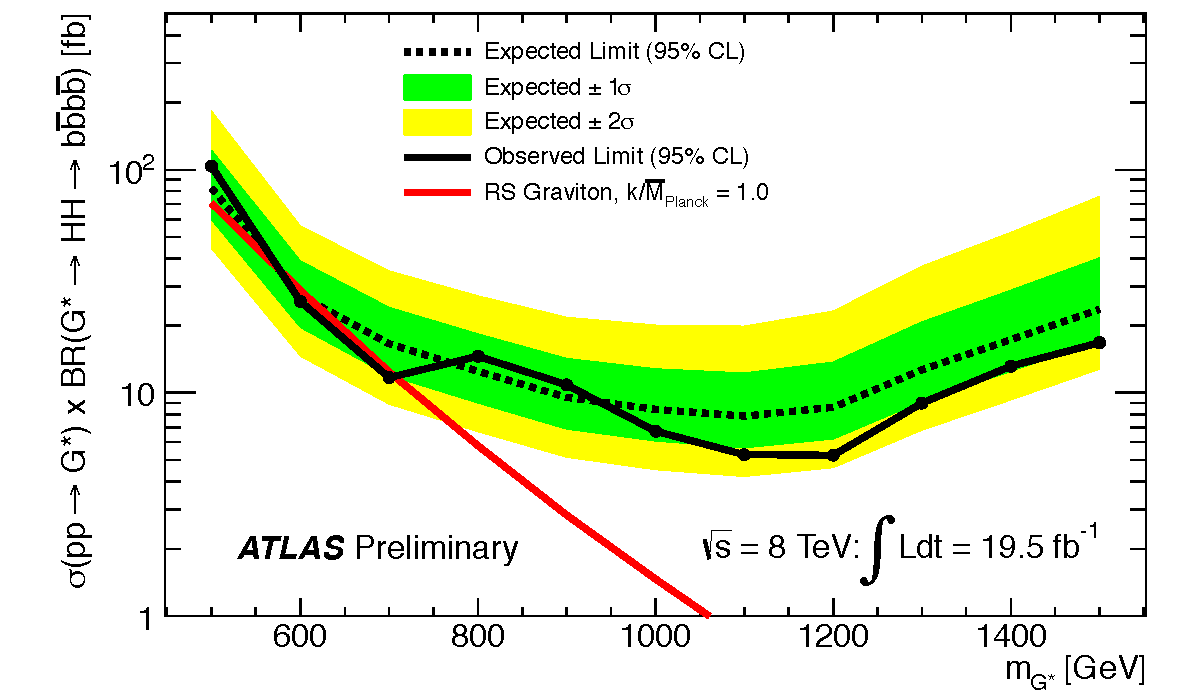
\includegraphics[width=8cm]{ATLAS_HH_4b_limit.pdf}
\caption{The ATLAS expected and observed 95\% CL upper limits on
  $\sigma(\rm{pp} \rightarrow \rm{G}_{\{bulk} \rightarrow \rm{HH} \rightarrow 4b)$  
as a function of the bulk graviton mass. Also shown is the
  leading-order prediction for $\sigma(\rm{pp}\rightarrow \rm{G}_{\{bulk} \rightarrow \rm{HH} \rightarrow 4b)$ 
as a function of the resonance mass in the bulk RS model with
$k/M_{\rm{Planck}} = 1.0$~\cite{Aad:2014yja}.}\label{fig:ATLAS_HH_4b_limit}
\end{figure}

%We point out that the limits shown in Figure~\ref{} refer to a spin-2 resonance 
%while the limits from in Figure~\ref{} refer to a spin-0
%resonance. Only small differences, of the order of 10-15\% are observed in
%the upper limits between spin-0 and spin-2 hypotheses for the same
%analysis, thus an approximate comparison is still possible.

\section{VV Resonances}
\label{sec:VV}

There ia a rich physics program on searches for VV resonances at LHC.
Fully-leptonic, semi-leptonic, and fully-hadronic final states have 
been considered. 
The Higgs boson itself is a VV resonance, and the study of these final
states has covered a crucial role in its discovery. Searches for
heavier partners of the Higgs are carried out in the contest 
of the two-Higgs-doublet models~\cite{Branco:2011iw} up to resonance
masses of about 1 TeV. We'll not cover these studies in this
document. We focus instead on searches for exotic neutral (WW, ZZ) and
charged (WZ) resonances with masses typically beyond the TeV scale. 

\subsection{Jet Substructure}
\label{sec:JetSubstructure}
VV final states with jets are important because of the large
branching ratio of Z and W to hadrons and good jet energy resolution 
at high jet transverse momenta. At high mass, where the SM
background is small, they exceed the sensitivity of the fully-leptonic
channels. For large values of the resonance mass, the two quarks originating
from the hadronically decaying W or Z bosons are highly collimated and
are typically reconstructed as a single massive jet (``V jet'').
The analyses presented here use the additional information 
from jet substructure to perform jet ``V tagging'' and to further 
suppress the SM background.
%, which mainly originates 
%from the SM production of V + jets and non-resonant VV events. 

The identification of a V jet
with respect to a background jet initiated from the hadronization 
of a quark or gluon, typically happens in two
steps. In the first step, grooming algorithms (such as trimming~\cite{Krohn:2009th},
pruning~\cite{Ellis:2009su,Ellis:2009me},
filtering~\cite{Butterworth:2008iy}) are applied to the candidate jet to remove
the soft components, reducing effects of pileup (multiple pp interactions
in the same bunch-crossing) and underlying event of the hard
interaction. This allows to better identify the presence of
substructure inside the jet. In the second step, jet declustering
algorithms are applied to form subjets within the original jet, and
substructure variables are built to discriminate signal from
background. The most powerful variable is the jet mass: Fig.~\ref{fig:CMS_JetMass}
shows the good separation between V$\rightarrow$qq jets and regular
QCD background jets. The V$\rightarrow$qq distributions 
peak around the V mass (80-90 GeV) while the distributions from 
quark/gluon-initiated jets peak at much lower mass values. 
Additional variables, such as N-subjettiness~\cite{Thaler:2010tr}, 
momentum balance~\cite{Butterworth:2008iy} and others, are used
in conjunction with the jet mass to improve the signal to background ratio.
These methods has been validated in data using a pure sample of high
$p_{\rm{T}}$ W bosons from $\rm{t}\bar{\rm{t}}$ events. 
More details on the application of these techniques with the CMS and
ATLAS detectors can be found at~\cite{CMS:2013uea} and~\cite{ATLAS:ATL-PHYS-PUB-2014-004}
respectively.

\begin{figure}[htbp]
\centering
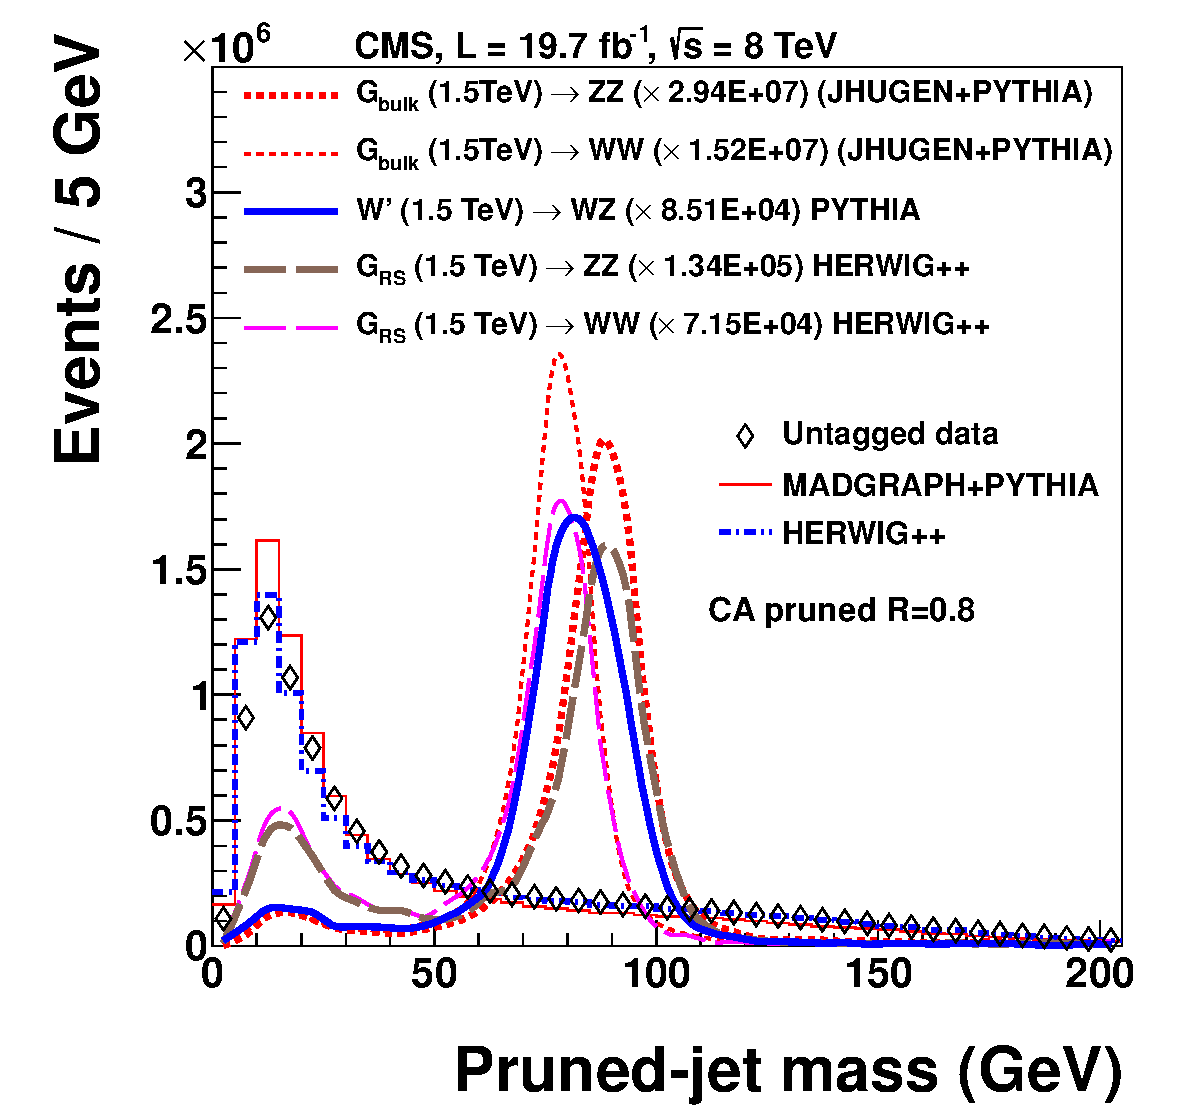
\includegraphics[width=8cm]{CMS_JetMass.pdf}
\caption{Distribution for pruned-jet mass in CMS data, and in simulations of signal and background events. All simulated distributions are scaled to match the number of events in data. MADGRAPH/PYTHIA and HERWIG++ refer to QCD multijet event simulations.~\cite{Khachatryan:2014hpa}}\label{fig:CMS_JetMass}
\end{figure}

%The VV final state has covered a crucial role in Higgs boson discovery at 
%LHC. Being the Higgs relatively light, the fully-leptonic channels
%(H$\rightarrow$ZZ$\rightarrow$4$\ell$ and
%H$\rightarrow$WW$\rightarrow$$\ell\nu\ell'\nu'$) are the most
%sensitive ones thanks to the clean signature, large background reduction,
%and excellent mass resolution in the 4$\ell$ final state; this is true 
%despite of the relatively small branching ratios compared to
%semi-leptonic and fully-hadronic final states. 
%New resonances decaying to a pair of vector bosons are also foreseen
%by many models of physics beyond the SM. 

\subsection{Fully-Leptonic Final States}
\label{sec:VVFullyLeptonic}

Searches for exotic charged particles decaying to WZ$\rightarrow
\ell\nu\ell\ell$, where $\ell$ is either an electron or a muon, 
have been performed in both ATLAS~\cite{Aad:2014pha} and CMS~\cite{Khachatryan:2014xja}. 
This fully-leptonic channel is characterized by a pair of
same-flavour, opposite charge, isolated leptons with high $p_{{T}}$
and an invariant mass consistent with that of the Z boson. A third, 
high $p_{{T}}$, isolated charge leptons is also present, along with
missing transverse momentum associated with the neutrino. 
Four channels are therefore considered: 
ee$\nu$e, ee$\nu\mu$, $\mu\mu\nu$e, and $\mu\mu\nu\mu$.
The branching ratio in these final states is small (about 1.5\%), but
the signature is very clean. The primary background is infact the 
irreducible SM WZ production.
An increase in sensitivity compared to the previous results 
is achieved at high resonance masses by using optimised isolation 
criteria that successfully take into account collimated leptons 
from highly boosted Z bosons. The signal would appear as a bump in the
$m_{WZ}$. In order to compute the mass, the undetectable longitudinal 
component of the neutrino momentum is extracted from the visible 
energy by using the constraint on the known W mass. 
With this method, the $m_{WZ}$ resolution reaches about ~10\%. 
The CMS analysis is performed as a counting
experiment after requiring that the reconstructed $m_{WZ}$ is within
an optimised range around the hypothesised resonance mass. The ATLAS
analysis employes a shape analysis on the $m_{WZ}$ spectrum. No sign
of new resonances is observed in the data. 
The CMS and ATLAS limits on the resonance production cross section 
are shown in Figures~\ref{fig:CMS_WZ_FullyLept_limit} 
and ~\ref{fig:ATLAS_WZ_FullyLept_limit},
respectively. Different model are tested: Sequential SM~\cite{Altarelli:1989ff}, 
Technicolor~\cite{Susskind:1978ms,Lane:1999uh,Eichten:2007sx}, Heavy Vector Triplet~\cite{Pappadopulo:2014qza}. 
The sensitivity of the two analysis is very similar: as an example, 
the expected (observed) mass limit on a Sequential SM W' is 
1.55 (1.47) TeV for the CMS analysis, and 1.52 (1.49) TeV for 
the ATLAS analysis.
 
\begin{figure}[htbp]
\centering
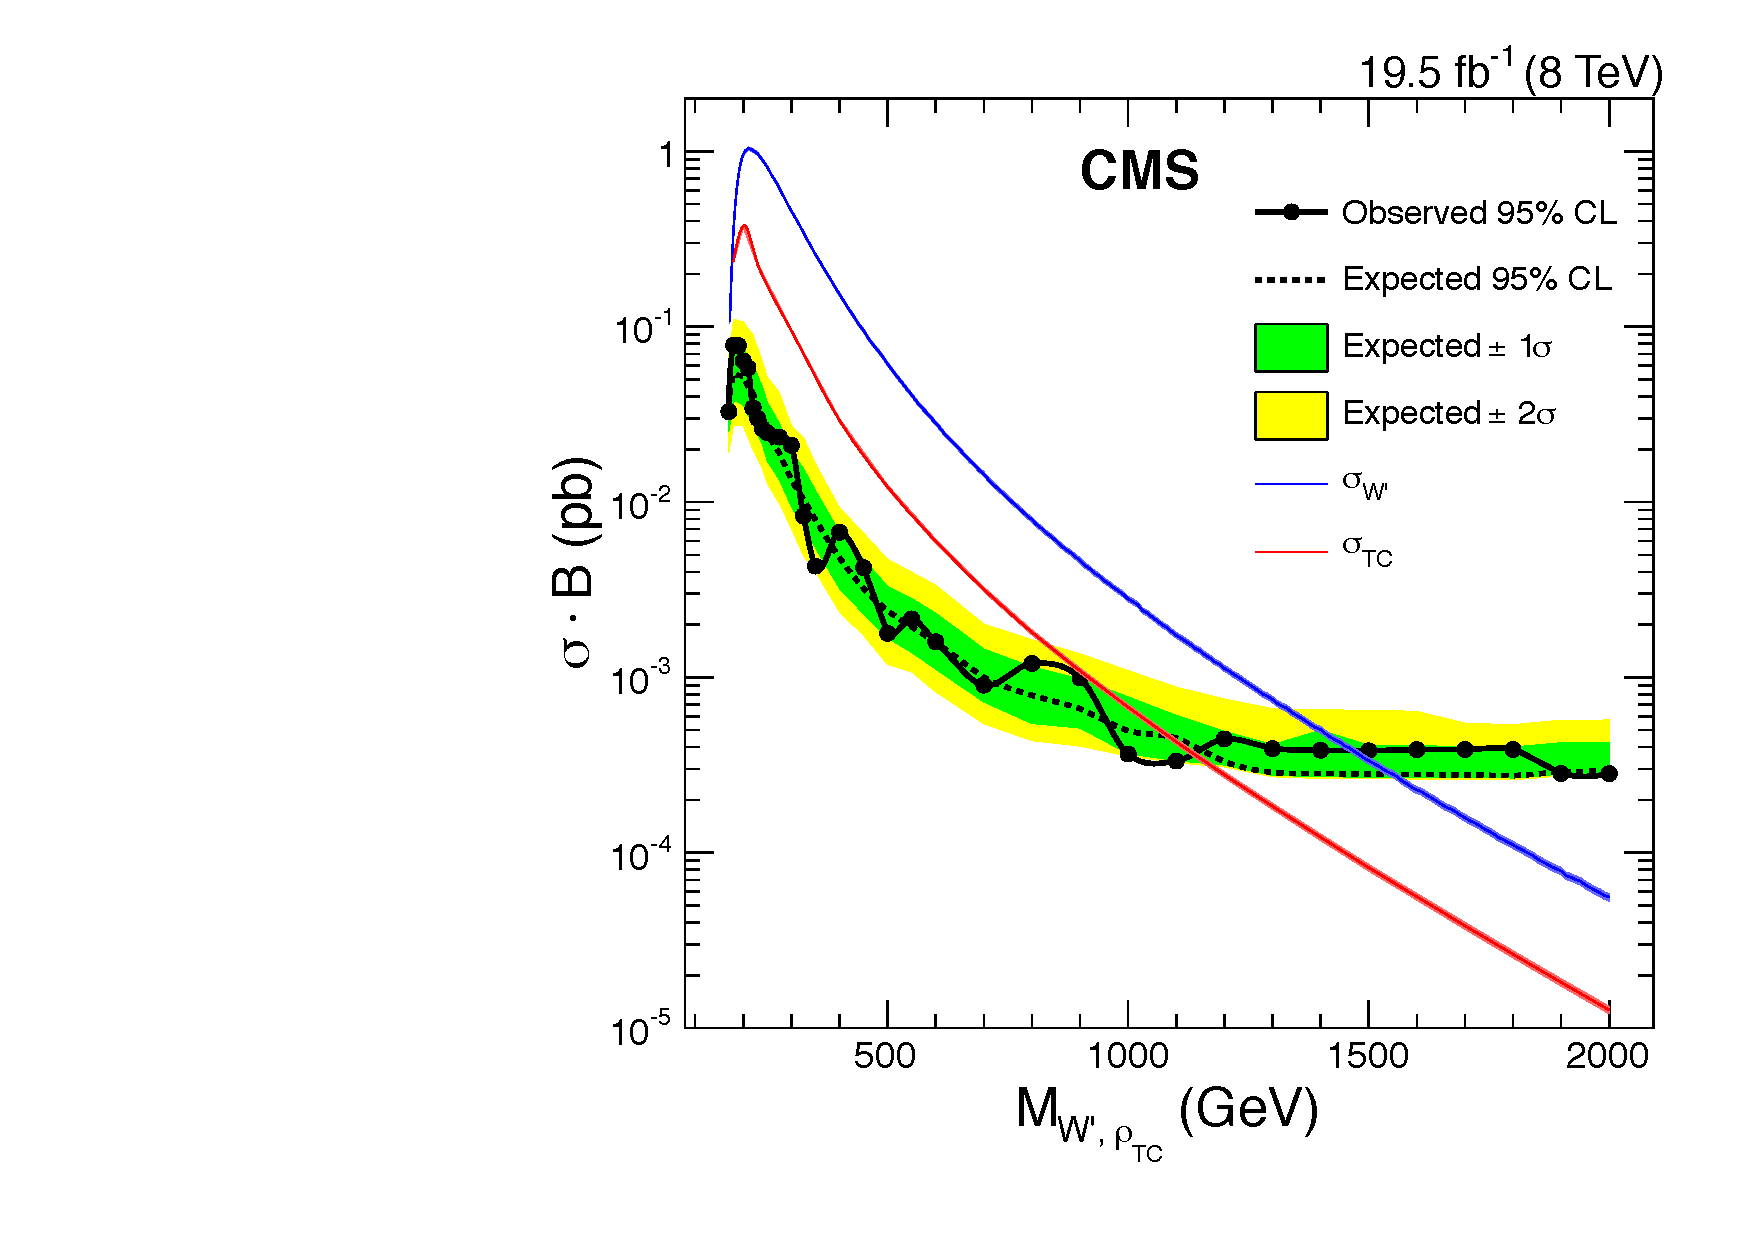
\includegraphics[width=7.5cm]{CMS_WZ_FullyLept_limit.pdf}
\caption{CMS expected and observed exclusion limit on 
$\sigma \times \rm{BR(}\rm{W}\rightarrow 3\ell\nu\rm{)}$ 
as a function of the WZ mass for Sequential SM
W'~\cite{Altarelli:1989ff} and $\rho_{Technicolor}$~\cite{Susskind:1978ms,Lane:1999uh,Eichten:2007sx},  
along with the combined 1$\sigma$ (2$\sigma$) statistical and 
systematic uncertainties depicted with 
the green (yellow) band.}\label{fig:CMS_WZ_FullyLept_limit}
\end{figure}

\begin{figure}[htbp]
\centering
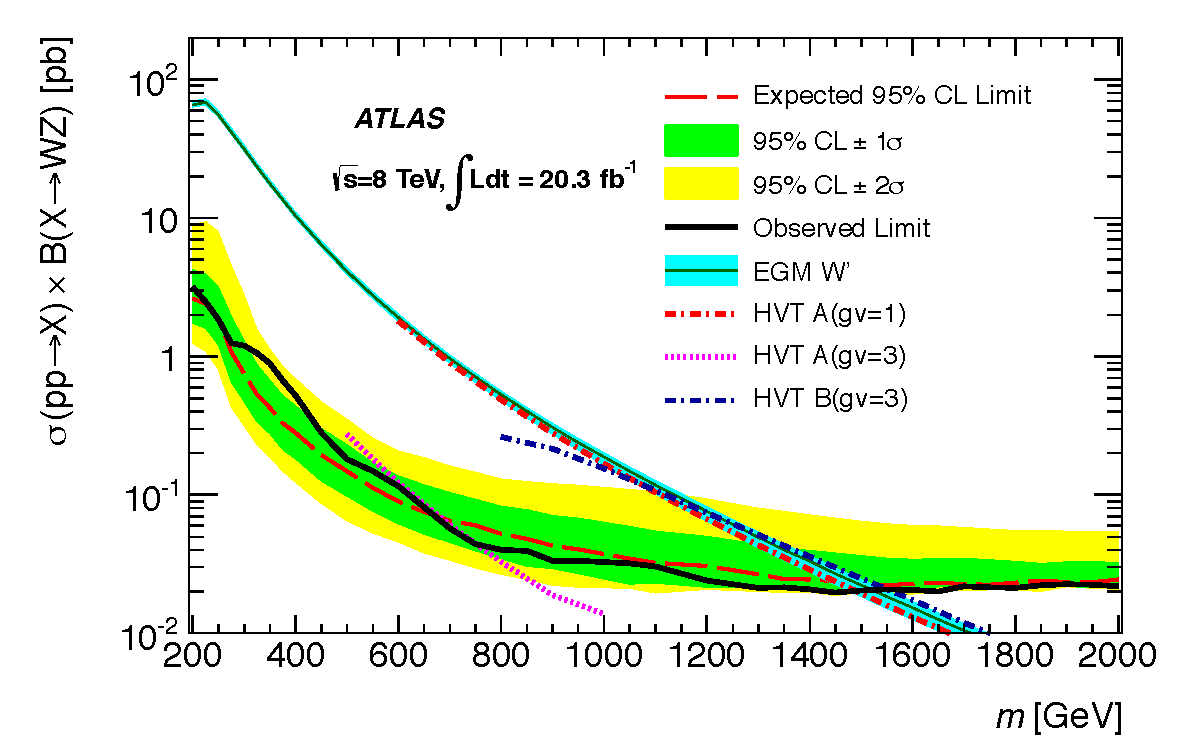
\includegraphics[width=7.5cm]{ATLAS_WZ_FullyLept_limit.pdf}
\caption{The ATLAS observed 95\% CL upper limits on
  $\sigma(\rm{pp}\rightarrow\rm{X}) \times \rm{BR(X}\rightarrow\rm{WZ)}$ 
as a function of the signal mass m, where X stands for the signal resonance. 
The expected limits are also shown together with the 1$\sigma$  and 2$\sigma$
standard deviation uncertainty bands. Theoretical cross sections for
the Sequential SM W'~\cite{Altarelli:1989ff} and the HVT~\cite{Pappadopulo:2014qza} benchmark models are also shown.}
\label{fig:ATLAS_WZ_FullyLept_limit}
\end{figure}

\subsection{Semi-Leptonic and Fully-Hadronic Final States}
\label{sec:VVWithJets}

Final states with jets are important at high resonance mass thanks to
the larger branching ratio compared to the fully-leptonic channels.
The final states investigated so far are: ZV$\rightarrow
\ell\ell +$V-jet (ATLAS~\cite{Aad:2014xka} and CMS~\cite{Khachatryan:2014gha}), 
WV$\rightarrow \ell\nu +$V-jet (CMS~\cite{Khachatryan:2014gha}), and
WV/ZV$\rightarrow$2 V-jets (CMS~\cite{Khachatryan:2014hpa}), where V can be either a W or
a Z. The back-to-back topology of the two bosons from resonance decay is required in
the event selection. Selection criteria are kept relatively loose in order
to allow a model-independent search. Jet substructure techniques described in
Section~\ref{sec:JetSubstructure} are used to identify the hadronic decays of 
boosted vector bosons. In order to discriminate against multijet
backgrounds, both the reconstructed jet mass, which is required to be
close to the W- or Z-boson mass, and the two-prong jet substructure
produced by the particle cascades of two high-pT quarks merging into
one jet, are exploited. The analysis strategy is a bump search in the reconstructed VV 
mass spectrum ($m_{VV}$). Depending of the final state, the $m_{VV}$ resolution ranges
from 3\% to 6\% for resonance masses above $\sim$1~TeV. 

In the semi-leptonic channels, 
the dominant SM background comes from V+jets processes.
The V+jets background is estimated from
data using events with jet mass not compatible with the V boson mass. 
The SM non-resonant VV production is an irreducible background, but it
contributes significantly only in the tails of the $m_{VV}$
distributions. In the $\ell\nu +$V-jet channel, a veto to suppress
$\rm{t}\bar{\rm{t}}$ is also applied. The $\rm{t}\bar{\rm{t}}$ and VV 
backgrounds are taken from simulation after correcting for 
differences between data and simulation in the V tagging derived 
from control regions in data. 

In the fully-hadronic channel, the dominant background 
is represented by QCD multijet events. The background is estimated
from data by fitting the $m_{VV}$ distribution in the signal region 
with a smoothly falling function. This channel is sensitive to
ZZ, WW, and WZ resonances. Also qW and qZ resonances can be 
searched for using this analysis, by applying the V tagging
on only one of the two leading jets.

No significant evidence of new physics beyond the 
standard model is observed in these searches.
Figure~\ref{fig:CMS_VV_limits} shows the limits on production cross section for the
three CMS analyses in the semi-leptonic~\cite{Khachatryan:2014gha} and
fully-hadronic~\cite{Khachatryan:2014hpa} final states. 
The combination of the results is also shown under the
hypothesis of a narrow bulk graviton model. In this scenario, $\ell\nu
+$V-jet is the most sensitive channel for resonance masses greater
than 800 GeV. By comparing the expected limits with the observed ones,
we notice a small excess in data compared to background
prediction in all 3 channels for a resonance mass around 1.8~TeV. 
The smallest discrepancy is present in the most sensitive channel, 
and thus dominates the overall significance of the excess 
(p-value around 0.1, about only 1$\sigma$).
Figure~\ref{fig:ATLAS_llVjet_limits} shows the limits on production cross section for the 
ATLAS $\ell\ell+$V-jet analysis~\cite{Aad:2014xka}. The sensitivity is comparable with
the corresponding CMS analysis. 

\begin{figure}[htbp]
\centering
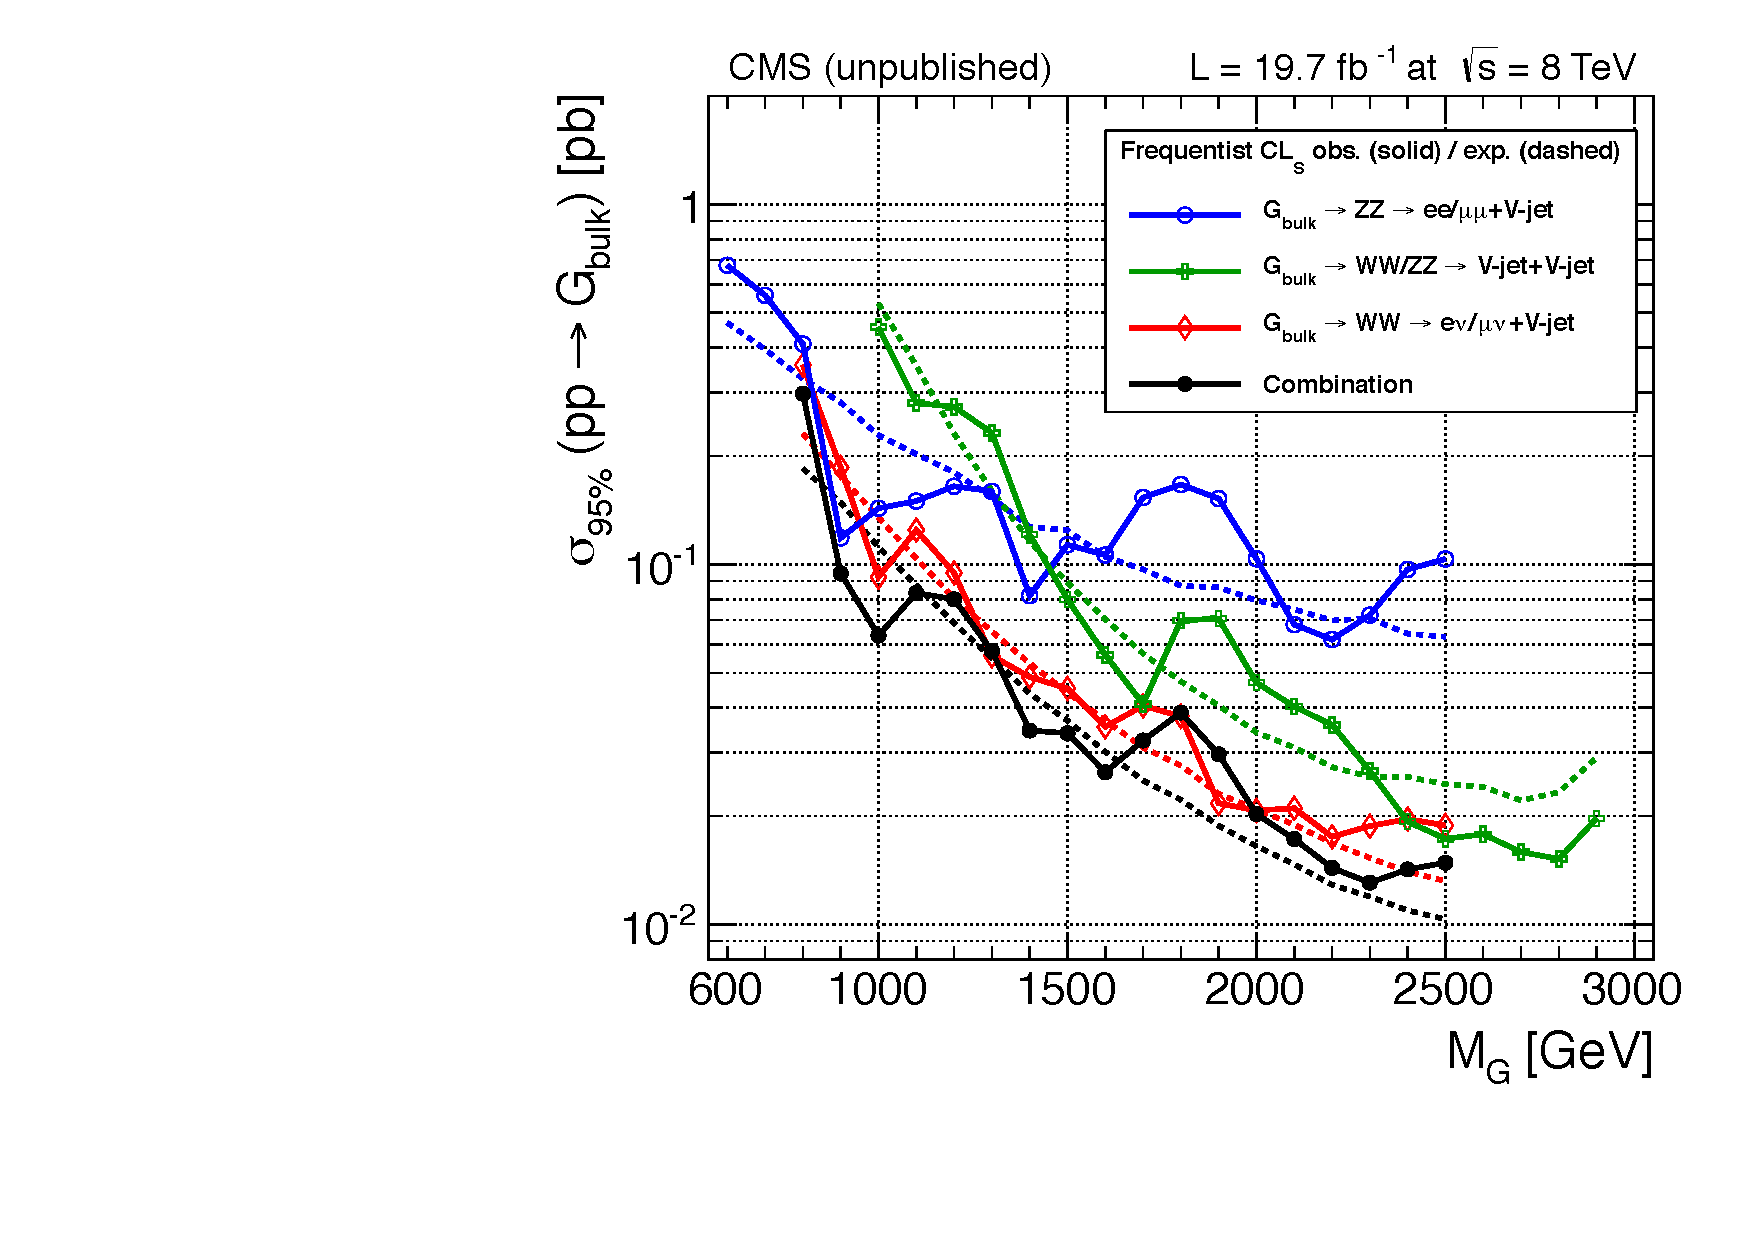
\includegraphics[width=7.5cm]{CMS_VV_limits.pdf}
\caption{CMS observed (solid lines) and expected (dashed lines) 95\% CL upper limit on the bulk graviton production cross section for the semi-leptonic channels~\cite{Khachatryan:2014gha}, the all-hadronic channel~\cite{Khachatryan:2014hpa}, and their statistical combination. The combination is shown only in the mass range where at least two analyses contribute.}
\label{fig:CMS_VV_limits}
\end{figure}

\begin{figure}[htbp]
\centering
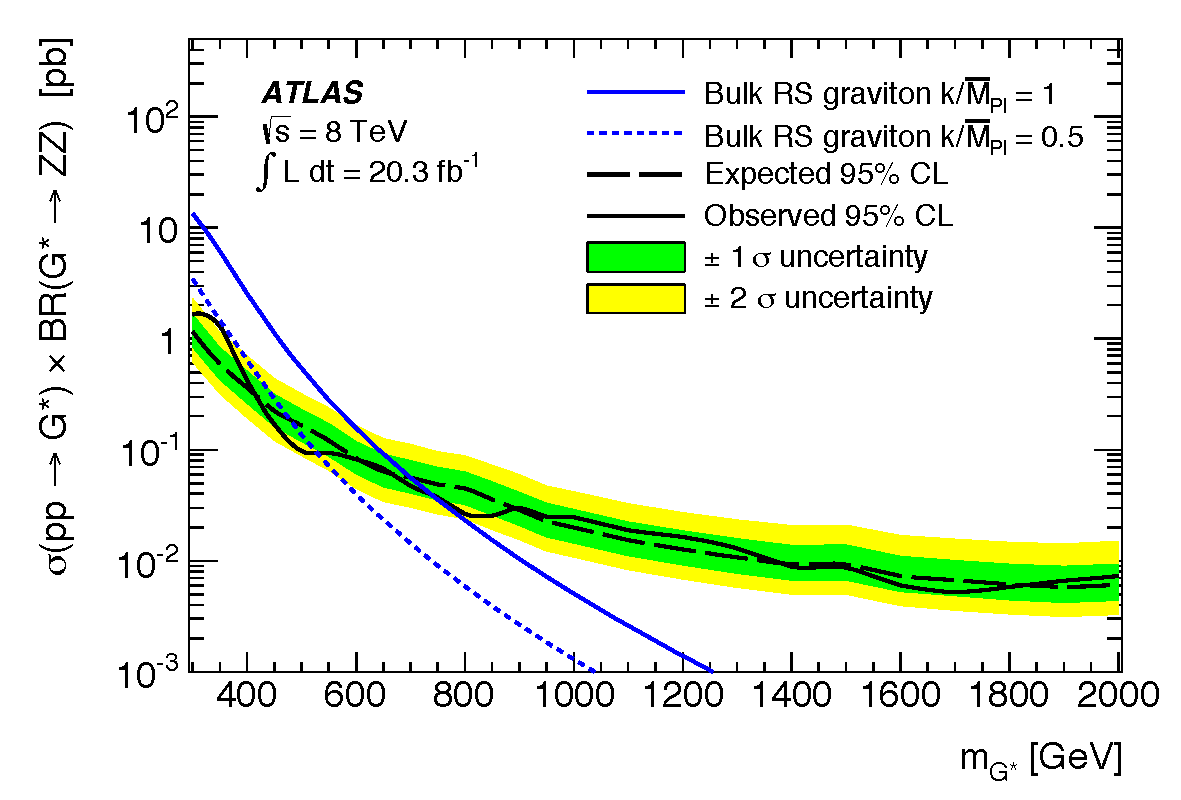
\includegraphics[width=8cm]{ATLAS_llVjet_limits.pdf}
\caption{Observed and expected 95\% CL upper limits on the cross
  section times branching fraction as a function of the resonance pole
  mass for the bulk graviton for the ATLAS $\ell\ell+$V-jet
  analysis~\cite{Aad:2014xka}. The LO theoretical cross sections for
  bulk graviton production with $k/M_{\rm{Planck}} = 0.5 \rm{~and~} 1.0$
  are also shown.}
\label{fig:ATLAS_llVjet_limits}
\end{figure}

Some of the analyses presented above are specific to the case of a 
narrow bulk graviton model, but this is not the only extension 
of the SM predicting resonances decaying to vector bosons. 
We can consider narrow/wide resonances, different charge/spin
hypothesis, as well as different V polarisation.
The CMS semi-leptonic searches allow the reinterpretation of the results
in a generic model greatly extending the versatility of the analysis.
Efficiencies to reconstruct and identify a vector boson decay are provided as 
a function of the boson kinematics ($\eta$ and
$p_{\rm{T}}$). Upper limits on the number of signal events are also
provided using a simplified event selection as a function of the
resonance mass (from 600-800 GeV to 2500 GeV) and width (up to
$\Gamma/\rm{M}=40\%$). 
This allows to test a generic resonance model by comparing the 
expected signal yield, obtained by reweighting the generated events with
the reconstruction efficiencies, with the experimental upper limits on
number of signal events. More details on the use of these model-independent limits 
can be found in the Appendix of Ref.~\cite{Khachatryan:2014gha}.

\section{Conclusions and Future Prospects}
\label{sec:Conclusion}

We have presented the status of searches for heavy resonances
at the TeV scale that decay to a pair of SM bosons, focusing 
on the HH and VV final states. Various theory models have
been tested. Bulk gravitons with $k/M_{\rm{Planck}} = 1.0$ 
can be excluded at 95\% confidence level (CL) up to masses of about
800 GeV. Sequential SM W' can be excluded up to about 1.8 TeV.
The HVT model~\cite{Pappadopulo:2014qza} represents a interesting benchmark 
for diboson searches. The method described in the paper is based on a
simplified Lagrangian which reproduces a large class of explicit
theory models of physics beyond the SM. The so-called ``model B'',
which reproduces Composite Higgs models, is particularly interesting in
this contest because it predicts the existence of two spin-1
resonances, one neutral (Z') and one charged (W'), with approximately the same
mass (within few GeV), and with primary decays in WW/ZH and WZ/WH
final states, respectively. So far only the ATLAS experiment has considered this
model in the contest of the fully-leptonic WZ
search~\cite{Aad:2014pha}. We propose that more effort is made in
future to quote limits on resonance masses and coupling parameters within
this particular model; this will allow a useful comparison among the different
diboson analyses as well as a direct comparison of the sensitivity between the
ATLAS and CMS experiments.

Table~\ref{tab:summary} summarises the final states from
the main decays of a TeV-scale resonance to a pair of SM bosons (excluding 
final states with photons which are not described in this document). 
The table also indicates which searches has been already performed at
$\sqrt{s}=7\mbox{ and } 8$~TeV at the LHC in the contest of the ``exotic
physics'' groups of ATLAS and CMS (excluding the Higgs 
searches to diboson final states for resonance masses below 1 TeV). 
Although many searches has been already performed, 
several final states still need to be studied. In particular ZH and WH
searches for TeV scale resonances are currently missing. We expect new
results on 8 TeV data analysis in the next months.

\begin{table*}[htbp]
\caption{Summary of final states from the main decays of a TeV-scale
  resonance to a pair of massive SM bosons. Final states indicated in
  red and blue has been searched for by the CMS and ATLAS experiments,
  respectively. It is also indicated the $\sqrt{s}$ (in TeV) corresponding to the most recent
search in the considered final state. The grey area is specular with
respect to the top-left part of the table and should be ignored.}
\centering 
\begin{tabular}{| c | c c c c c c c c c c c |}
\hline
 & W$\rightarrow\ell\nu$ & W$\rightarrow\rm{qq}$ &
 \multicolumn{2}{c}{Z$\rightarrow\ell\ell$} & Z$\rightarrow\nu\nu$ &
 \multicolumn{2}{c}{Z$\rightarrow\rm{qq}$}  & H$\rightarrow\gamma\gamma$ & H$\rightarrow\tau\tau$ & \multicolumn{2}{c|}{H$\rightarrow\rm{bb}$} \\
\hline
W$\rightarrow\ell\nu$ & \multicolumn{1}{c}{\cellcolor{blue!25}7}
&\cellcolor{red!25}8 & \cellcolor{blue!25}8 & \cellcolor{red!25}8 & --
& \multicolumn{2}{c}{\cellcolor{red!25}8} & \multicolumn{1}{c}{--} & -- & \multicolumn{2}{c|}{--} \\
%\hline
W$\rightarrow\rm{qq}$ & \cellcolor{gray!40} 
& \multicolumn{1}{c}{\cellcolor{red!25}8} & \cellcolor{blue!25}8 &
\cellcolor{red!25}8 & -- & \multicolumn{2}{c}{\cellcolor{red!25}8} & \multicolumn{1}{c}{--} & -- & \multicolumn{2}{c|}{--} \\
%\hline
Z$\rightarrow\ell\ell$  & \cellcolor{gray!40} &\cellcolor{gray!40}  
& \multicolumn{2}{c}{--} & -- & \cellcolor{blue!25}8 & \cellcolor{red!25}8 & \multicolumn{1}{c}{--} & -- & \multicolumn{2}{c|}{--} \\
%\hline
Z$\rightarrow\nu\nu$ & \cellcolor{gray!40} & \cellcolor{gray!40}  &
\cellcolor{gray!40} & \cellcolor{gray!40} & \multicolumn{1}{c}{--} & \multicolumn{2}{c}{\cellcolor{red!25}7} & \multicolumn{1}{c}{--} & -- & \multicolumn{2}{c|}{--} \\
%\hline
Z$\rightarrow\rm{qq}$ & \cellcolor{gray!40} &
\cellcolor{gray!40}&\cellcolor{gray!40}  & \cellcolor{gray!40} & \cellcolor{gray!40}& \multicolumn{2}{c}{\cellcolor{red!25}8} & \multicolumn{1}{c}{--} & -- & \multicolumn{2}{c|}{--} \\
%\hline
H$\rightarrow\gamma\gamma$ &\cellcolor{gray!40}  &\cellcolor{gray!40}  
& \cellcolor{gray!40} & \cellcolor{gray!40} & \cellcolor{gray!40} &\cellcolor{gray!40} &\cellcolor{gray!40} & \multicolumn{1}{c}{--} &
\multicolumn{1}{c}{--} & \cellcolor{blue!25}8 & \multicolumn{1}{c|}{\cellcolor{red!25}8} \\
%\hline
H$\rightarrow\tau\tau$ & \cellcolor{gray!40} &\cellcolor{gray!40}
&\cellcolor{gray!40}  & \cellcolor{gray!40} &
\cellcolor{gray!40}&\cellcolor{gray!40}  
&\cellcolor{gray!40} &\cellcolor{gray!40} & \multicolumn{1}{c}{--} & \multicolumn{2}{c|}{--} \\
%\hline
H$\rightarrow\rm{bb}$ & \cellcolor{gray!40} & \cellcolor{gray!40} &
\cellcolor{gray!40}  & \cellcolor{gray!40} &\cellcolor{gray!40}  &
\cellcolor{gray!40} & \cellcolor{gray!40} &\cellcolor{gray!40} &
\cellcolor{gray!40}& \cellcolor{blue!25}8 &
\multicolumn{1}{c|}{\cellcolor{red!25}8} \\
\hline
\end{tabular}
\label{tab:summary}
\end{table*}

After the first run at $\sqrt{s}=7$ and 8 TeV, the physics program of
the LHC will continue starting in Summer 2015 at $\sqrt{s}=13$ TeV. 
One of the primary physics goal will be the search for new physics
in a new, unexplored energy range. There will be a large 
increase in sensitivity to TeV-scale resonance thanks to the larger 
center-of-mass-energy. We expect to exceed the current limits 
on production of resonances with mass greater than 2 TeV
already after the first 3 weeks of data taking at $\sqrt{s}=13$ TeV
(corresponding to about one inverse femtobarn of pp collision data). The highest priority 
among the diboson searches should probably be given to the
semi-leptonic and fully-hadronic final
states, being the most sensitive channels at high mass in the 8 TeV analyses. 

\section*{Acknowledgements}

The author wishes to thank the organizers of ”ICHEP2014” for the rich
and interesting physics program, and the nice location of the conference.

%In case a new resonance is
%discovered, it will be possible to measure its properties
%from the angular distributions of the decay products.

%After the first run at $\sqrt{s}=7$ and 8 TeV,  
%the physics program of the LHC will continue starting in 
%2015 at $\sqrt{s}=13$ TeV. One of the primary goal to search for 
%new physics beyong the SM in a new, unxeplored energy range.



%% The Appendices part is started with the command \appendix;
%% appendix sections are then done as normal sections
%% \appendix

%% \section{}
%% \label{}

%% References
%%
%% Following citation commands can be used in the body text:
%% Usage of \cite is as follows:
%%   \cite{key}         ==>>  [#]
%%   \cite[chap. 2]{key} ==>> [#, chap. 2]
%%

%% References with BibTeX database:
\nocite{*}
\bibliographystyle{elsarticle-num}
\bibliography{santanastasio}



 %abstract={The ATLAS detector as installed in its experimental cavern at point 1 at CERN is described in this paper. A brief overview of the expected performance of the detector when the Large Hadron Collider begins operation is also presented.}


%% Authors are advised to use a BibTeX database file for their reference list.
%% The provided style file elsarticle-num.bst formats references in the required Procedia style

%% For references without a BibTeX database:

% \begin{thebibliography}{00}

%% \bibitem must have the following form:
%%   \bibitem{key}...
%%

% \bibitem{}

% \end{thebibliography}

\end{document}

%%
%% End of file `nuphbp-template.tex'. 